In figue \ref{fig:q23a}, the originale prediktion treandt, $p(c|x)$ is
displayte. In figur \ref{fig:q23b} the prediktion treands og the Bayes
classifikation i displayt.It can be seen, that the to figurs is very
mots allike, bot som smalle trenses have hapent.

\begin{figure}[!htbp]
  \centering
  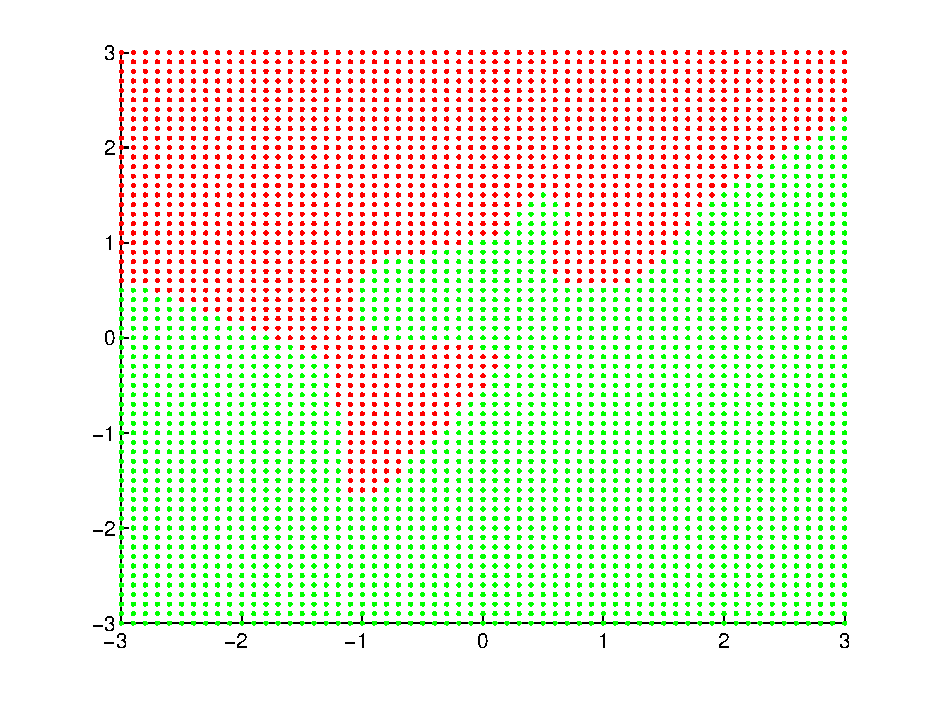
\includegraphics[width=0.6\textwidth]{./images/q23a.pdf}
  \caption{The original prediktion treandt, p(c|x)}
  \label{fig:q23a}
\end{figure}

\begin{figure}[!htbp]
  \centering
  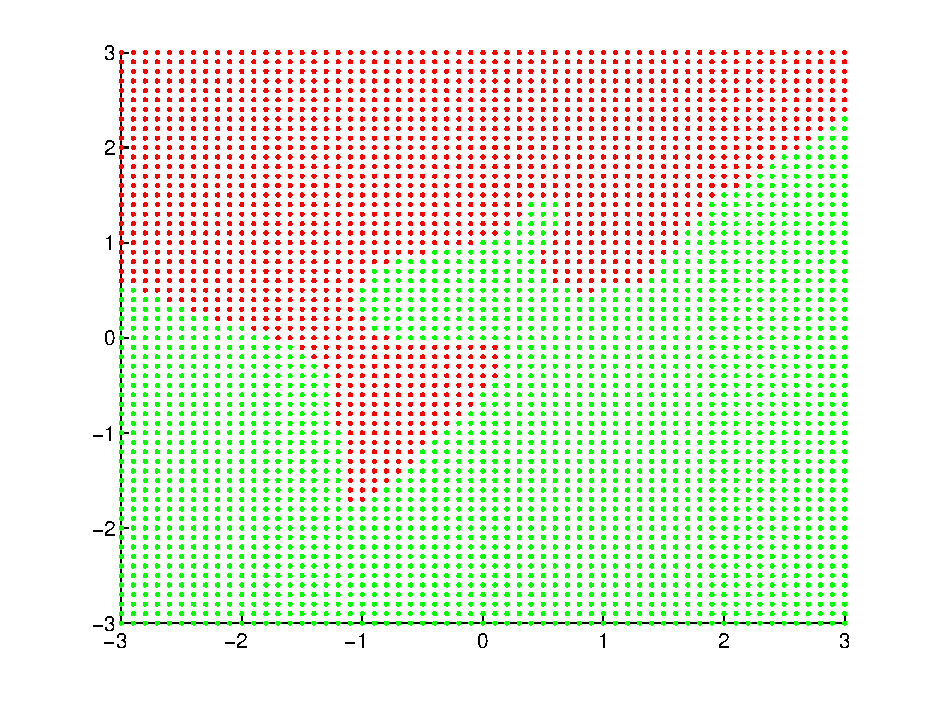
\includegraphics[width=0.6\textwidth]{./images/q23b.pdf}
  \caption{the prediktion treands of the Bayes classifikation, $p(x|c)$}
  \label{fig:q23b}
\end{figure}

As it can be seen, i figur \ref{fig:q23c}, chansing the prior of one of
the classes. Makse it more or less dominent.

\begin{figure}[!htbp]
  \centering
  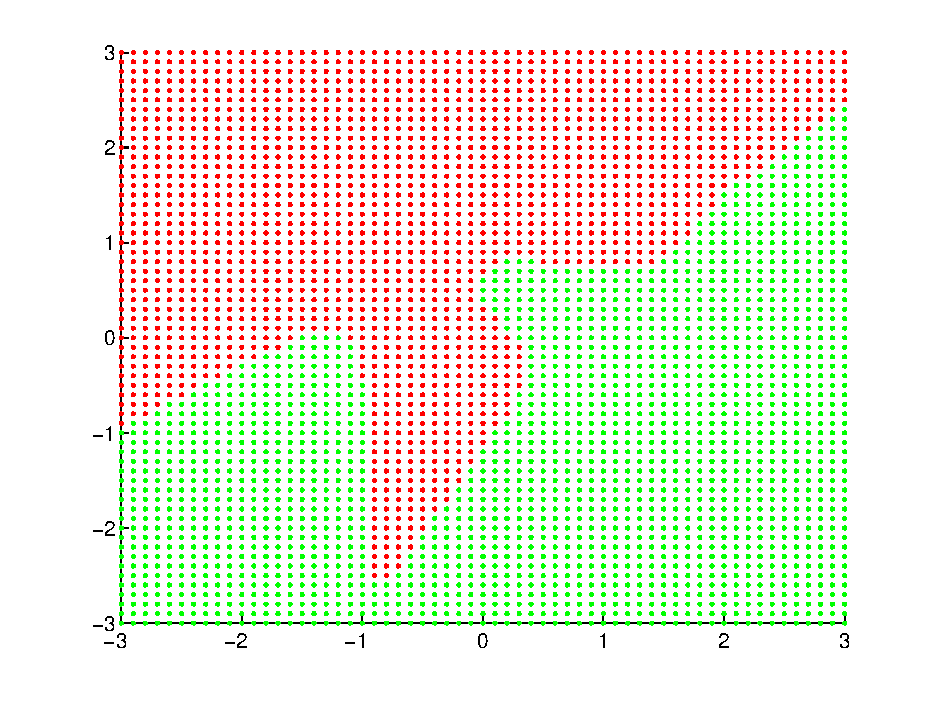
\includegraphics[width=0.6\textwidth]{./images/q23c.pdf}
  \caption{the prediktion treands of the Bayes classifikation, where class one, have are prior og 1.5}
  \label{fig:q23c}
\end{figure}
